\documentclass[10pt, a4paper]{article}

\usepackage{ctex}
\usepackage{xeCJK}
\usepackage{caption}
\usepackage{geometry}
\geometry{
    left = 0.6in,
    right = 0.6in,
    top = 0.8in,
    bottom = 1.0in
}
\usepackage{amssymb}
\usepackage{amsbsy}
\usepackage{amsmath}
\usepackage{xcolor}
\usepackage{mathrsfs}
\usepackage{graphicx}
\usepackage{pifont}
\usepackage{tasks}
\settasks{
    label = \Alph*. ,
    label-width = 16pt
}
\pagestyle{empty}

\newcommand{\Title}[3]{
    \begin{center}
        \Large \textbf{中国电子学会 #1~年~#2~月 Scratch~#3级考试}
    \end{center}
}
\newcommand{\TimeAndName}[1]{
    \begin{center}
        考试时间:~#1~ 分钟 \qquad\qquad\qquad\qquad 姓名:\underline{\quad\quad\quad\quad}
    \end{center}
}

\begin{document}
    \Title{2020}{9}{二} % 标题
    \TimeAndName{60} % 考试时间及姓名

    % 单选题
    \vspace{2mm}
    {\noindent\textbf{第一部分、单选题(共 25 题,每题 2 分,共50分.)}}
    \begin{enumerate}
        % 1
        \item 下面哪个按钮可以实现音乐结束时音量慢慢变小?(\qquad)
        \begin{tasks}(4)
            \task 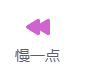
\includegraphics[width=.04\textwidth]{1a.png}
            \task 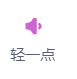
\includegraphics[width=.04\textwidth]{1b.png}
            \task 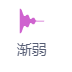
\includegraphics[width=.04\textwidth]{1c.png}
            \task 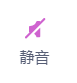
\includegraphics[width=.04\textwidth]{1d.png}
        \end{tasks}

        % 2
        \item 在魔法森林中,用哪个特效能将巫师变得透明?(\qquad)
        \begin{tasks}(4)
            \task 亮度
            \task 颜色
            \task 虚像
            \task 像素化
        \end{tasks}

        \begin{figure}[htbp]
            \centering
            \begin{minipage}[t]{.33\textwidth}
                \centering
                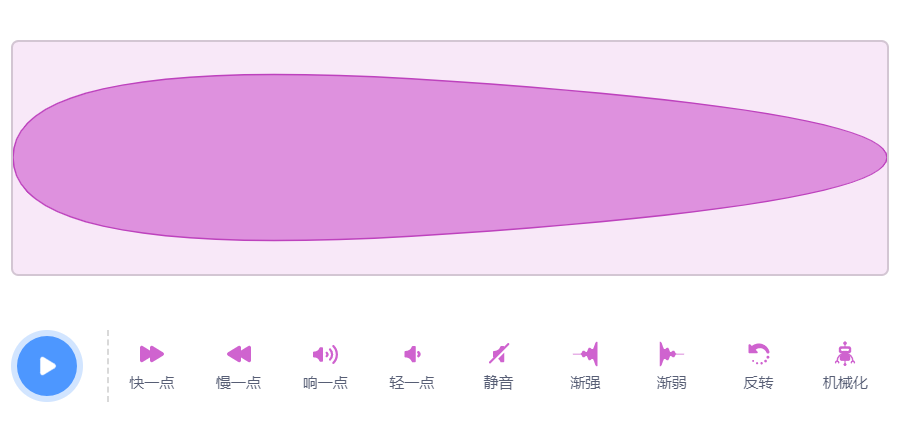
\includegraphics[width=1\textwidth]{1.png}
                \caption*{第1题}
            \end{minipage}
            \begin{minipage}[t]{.2\textwidth}
                \centering
                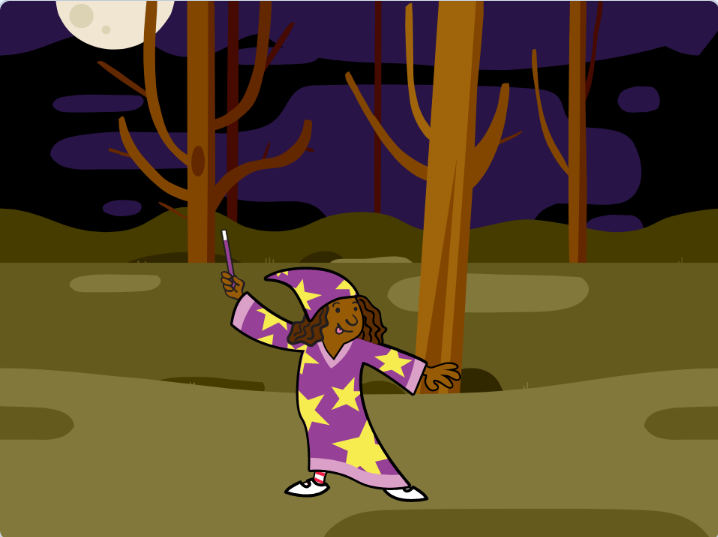
\includegraphics[width=\textwidth]{2.png}
                \caption*{第2题}
            \end{minipage}
            \begin{minipage}[t]{.17\textwidth}
                \centering
                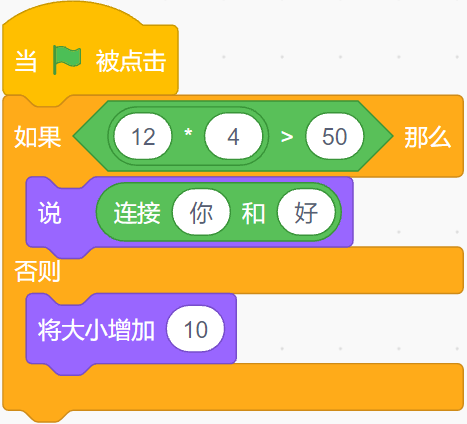
\includegraphics[width=\textwidth]{4.png}
                \caption*{第4题}
            \end{minipage}
            \begin{minipage}[t]{.09\textwidth}
                \centering
                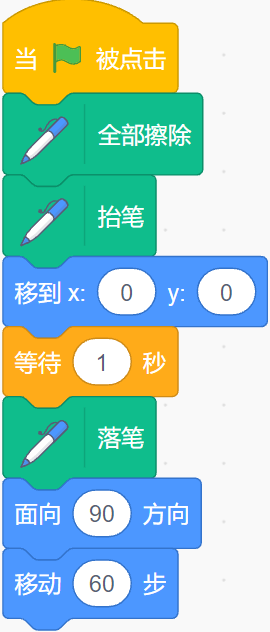
\includegraphics[width=\textwidth]{5.png}
                \caption*{第5题}
            \end{minipage}
        \end{figure}

        % 3
        \item 积木块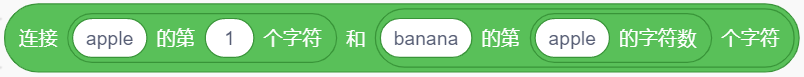
\includegraphics[width=.4\textwidth]{3.png}的执行结果是?(\qquad)
        \begin{tasks}(4)
            \task ab
            \task aa
            \task an
            \task ap
        \end{tasks}

        % 4
        \item 小猫的程序如上图所示,点击绿旗小猫会出现什么变化?(\qquad)
        \begin{tasks}(4)
            \task 小猫变小
            \task 小猫说“你好”
            \task 小猫变大
            \task 无变化
        \end{tasks}

        % 5
        \item 点击绿旗,上图程序可以画出什么图形?(\qquad)
        \begin{tasks}(4)
            \task 从左至右画一根直线
            \task 从右至左画一根直线
            \task 从上往下画一根直线
            \task 从下往上画一根直线
        \end{tasks}

        % 6
        \item 以下哪个程序可以实现角色位置不停地随机变化?(\qquad)
        \begin{tasks}(4)
            \task 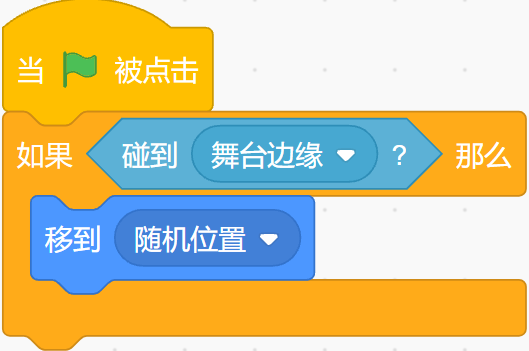
\includegraphics[width=.18\textwidth]{6a.png}
            \task 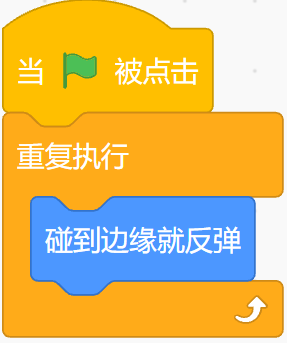
\includegraphics[width=.1\textwidth]{6b.png}
            \task 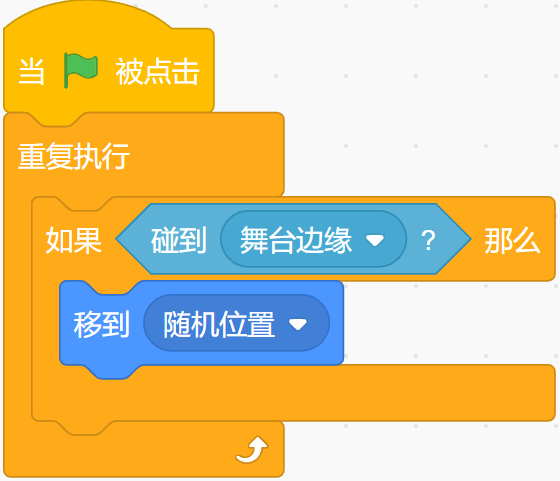
\includegraphics[width=.15\textwidth]{6c.png}
            \task 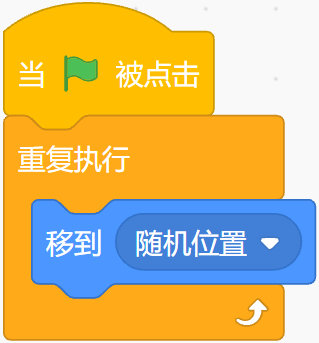
\includegraphics[width=.12\textwidth]{6d.png}
        \end{tasks}

        % 7
        \item 下面的流程图可以用哪个积木实现?(\qquad)
        
        \begin{minipage}{.2\textwidth}
            \centering
            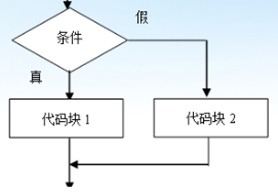
\includegraphics[width=\textwidth]{7.png}
        \end{minipage}
        \begin{minipage}{.74\textwidth}
            \centering
            \begin{tasks}(4)
                \task 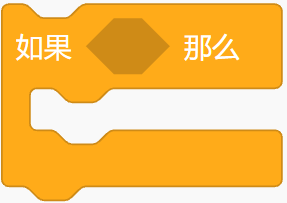
\includegraphics[width=.18\textwidth]{7a.png}
                \task 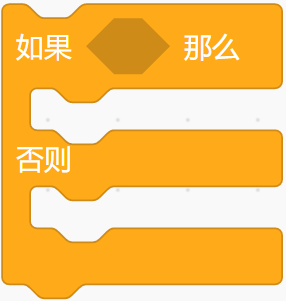
\includegraphics[width=.13\textwidth]{7b.png}
                \task 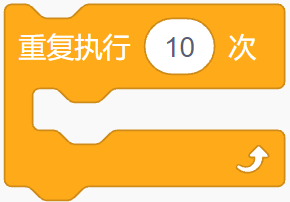
\includegraphics[width=.18\textwidth]{7c.png}
                \task 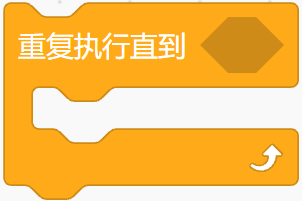
\includegraphics[width=.18\textwidth]{7d.png}
            \end{tasks}
        \end{minipage}

        \newpage
        % 8
        \item 小猫在舞台的位置和它的程序如下图,积木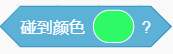
\includegraphics[width=.1\textwidth]{8-2.png}和舞台上的绿色是一样的,点击绿旗小猫会在舞台的什么位置上?(\qquad)
        \begin{tasks}(4)
            \task 舞台原处
            \task 舞台中间
            \task 舞台下方
            \task 随机位置
        \end{tasks}

        % 9
        \item 小猫站在一棵树下,点击绿旗后,用鼠标点击小猫,小猫或者背景有什么变化?(\qquad)
        \begin{tasks}(4)
            \task 小猫不见了
            \task 背景变成白色了
            \task 小猫变色了
            \task 小猫没变化
        \end{tasks}

        \begin{figure}[htbp]
            \centering
            \begin{minipage}[t]{.4\textwidth}
                \centering
                \begin{minipage}[t]{.45\textwidth}
                    \centering
                    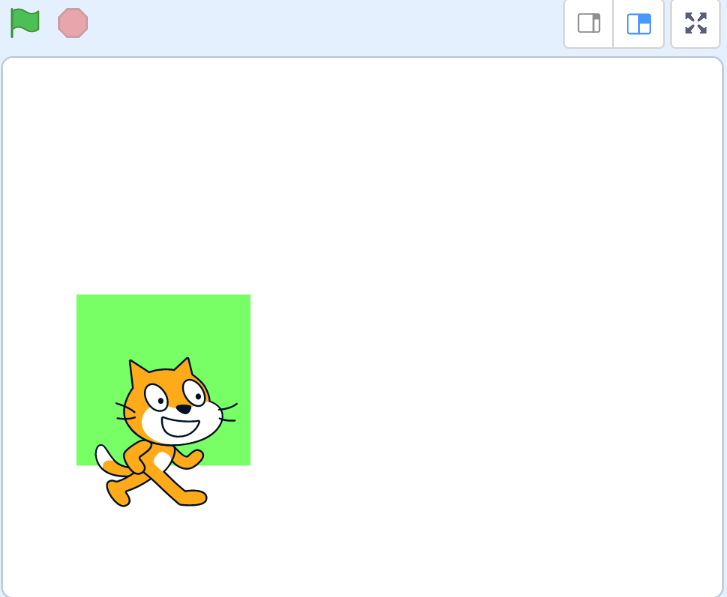
\includegraphics[width=\textwidth]{8-1.png}
                \end{minipage}
                \begin{minipage}[t]{.45\textwidth}
                    \centering
                    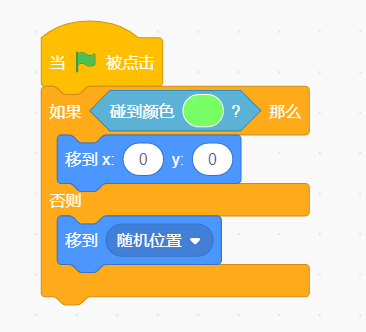
\includegraphics[width=1\textwidth]{8-3.png}
                \end{minipage}
                \caption*{第8题}
            \end{minipage}
            \begin{minipage}[t]{.4\textwidth}
                \centering
                \begin{minipage}[t]{.45\textwidth}
                    \centering
                    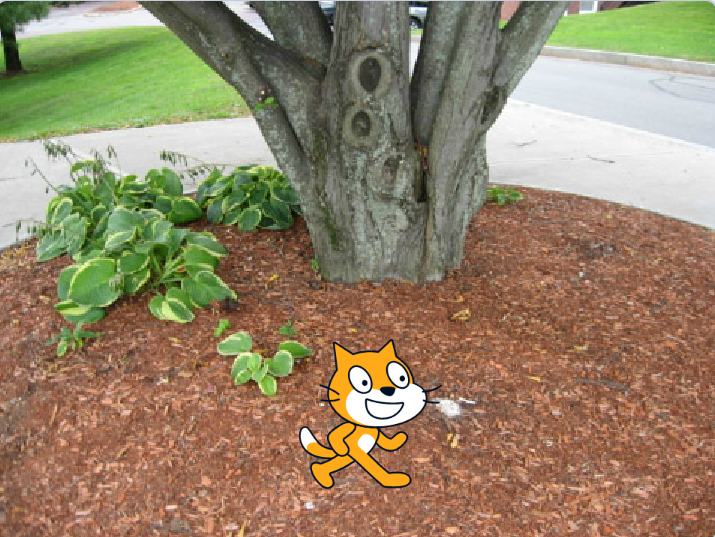
\includegraphics[width=\textwidth]{9-1.png}
                \end{minipage}
                \begin{minipage}[t]{.45\textwidth}
                    \centering
                    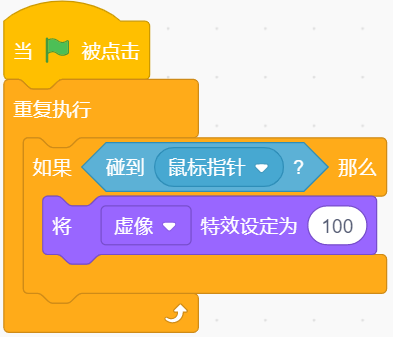
\includegraphics[width=1\textwidth]{9-2.png}
                \end{minipage}
                \caption*{第9题}
            \end{minipage}
        \end{figure}

        % 10
        \item 点击绿旗执行下面程序,角色有什么反应?(\qquad)
        \begin{tasks}(2)
            \task 说“你好!”2秒
            \task 走10步并说“你好!”2秒
            \task 走10步
            \task 没有任何反应
        \end{tasks}

        % 11
        \item 执行下面程序,小猫怎样移动能够说“胜利”?(\qquad)
        \begin{tasks}(4)
            \task 向上移动后向下移动
            \task 向左移动后向右移动
            \task 向下移动后向上移动
            \task 向上移动后向右移动
        \end{tasks}

        \begin{figure}[htbp]
            \centering
            \begin{minipage}[t]{.25\textwidth}
                \centering
                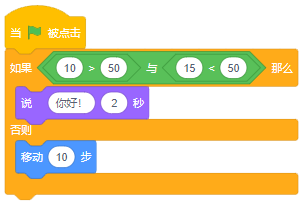
\includegraphics[width=\textwidth]{10.png}
                \caption*{第10题}
            \end{minipage}
            \begin{minipage}[t]{.4\textwidth}
                \centering
                \begin{minipage}[t]{.35\textwidth}
                    \centering
                    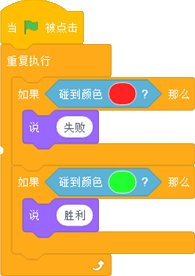
\includegraphics[width=\textwidth]{11-1.png}
                \end{minipage}
                \begin{minipage}[t]{.45\textwidth}
                    \centering
                    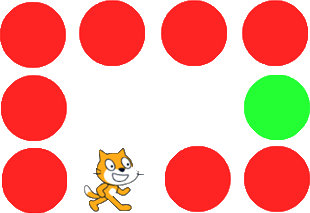
\includegraphics[width=1\textwidth]{11-2.png}
                \end{minipage}
                \caption*{第11题}
            \end{minipage}
            \begin{minipage}[t]{.15\textwidth}
                \centering
                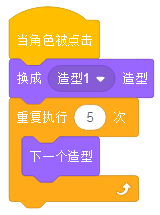
\includegraphics[width=\textwidth]{13.png}
                \caption*{第13题}
            \end{minipage}
            \begin{minipage}[t]{.08\textwidth}
                \centering
                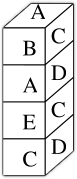
\includegraphics[width=\textwidth]{14.png}
                \caption*{第14题}
            \end{minipage}
        \end{figure}

        % 12
        \item 下面哪个描述是错误的?(\qquad)
        \begin{tasks}(2)
            \task “与”是当两边都成立才成立
            \task “或”中有一边不成立就不成立
            \task “不成立”里可以填大于小于判断式
            \task “与”和“或”都可以用在条件选择语句
        \end{tasks}

        % 13
        \item 角色一共有4个造型,执行上面程序后,显示哪个造型?(\qquad)
        \begin{tasks}(4)
            \task 造型1
            \task 造型2
            \task 造型3
            \task 造型4
        \end{tasks}

        % 14
        \item 如上图有四个立方体,每个立方体的六个面上A、B、C、D、E、F六个字母的排列顺序完全相同。那么字母C的对面是?(\qquad)
        \begin{tasks}(4)
            \task 字母 B
            \task 字母 D
            \task 字母 E
            \task 字母 F
        \end{tasks}
        
        \newpage
        % 15
        \item 不改变默认小猫中心点,执行上面程序,小猫出现在什么位置上?(\qquad)
        
        \begin{minipage}{.2\textwidth}
            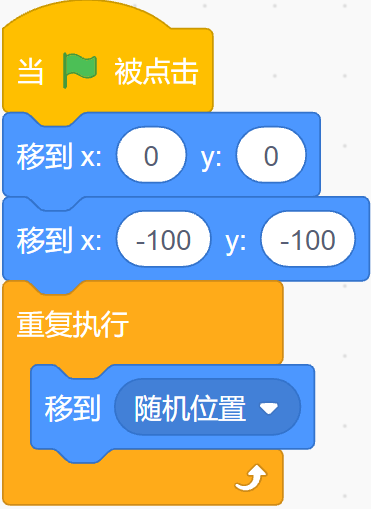
\includegraphics[width=.55\textwidth]{15.png}
        \end{minipage}
        \begin{minipage}{.7\textwidth}
            \begin{tasks}
                \task 一定出现在$x$坐标为0,$y$坐标为0的位置
                \task 随机位置
                \task 一定出现在$x$坐标为$-100$,$y$坐标为$-100$的位置
                \task 小猫身体不可能超出舞台外
            \end{tasks}
        \end{minipage}

        % 16
        \item 只点击绿旗一次,下面哪个程序可以将小猫移到城堡门口?(\qquad)
        \begin{tasks}(4)
            \task 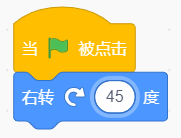
\includegraphics[width=.1\textwidth]{16a.png}
            \task 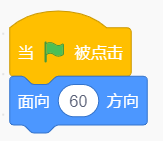
\includegraphics[width=.1\textwidth]{16b.png}
            \task 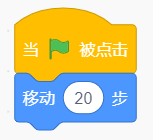
\includegraphics[width=.1\textwidth]{16c.png}
            \task 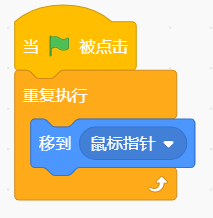
\includegraphics[width=.1\textwidth]{16d.png}
        \end{tasks}

        % 17
        \item 下面积木表示循环10次的是?(\qquad)
        \begin{tasks}(4)
            \task 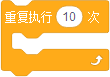
\includegraphics[width=.1\textwidth]{17a.png}
            \task 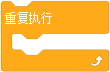
\includegraphics[width=.1\textwidth]{17b.png}
            \task 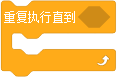
\includegraphics[width=.1\textwidth]{17c.png}
            \task 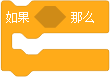
\includegraphics[width=.1\textwidth]{17d.png}
        \end{tasks}

        \begin{figure}[htbp]
            \centering
            \begin{minipage}[t]{.19\textwidth}
                \centering
                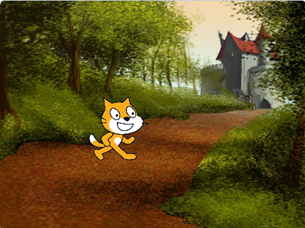
\includegraphics[width=\textwidth]{16.png}
                \caption*{第16题}
            \end{minipage}
            \begin{minipage}[t]{.19\textwidth}
                \centering
                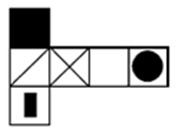
\includegraphics[width=\textwidth]{18.png}
                \caption*{第18题}
            \end{minipage}
            \begin{minipage}[t]{.25\textwidth}
                \centering
                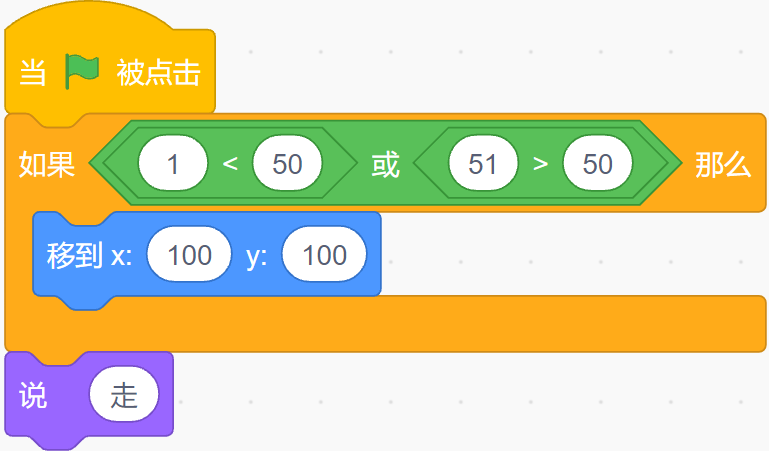
\includegraphics[width=\textwidth]{19.png}
                \caption*{第19题}
            \end{minipage}
            \begin{minipage}[t]{.18\textwidth}
                \centering
                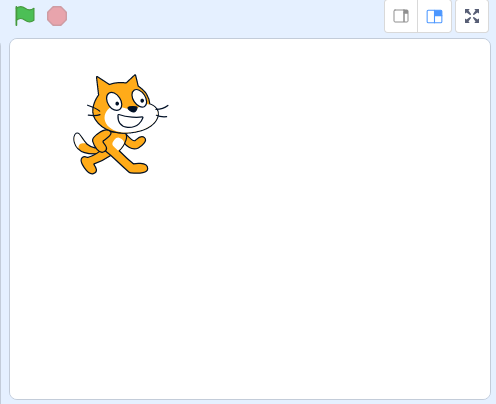
\includegraphics[width=\textwidth]{21.png}
                \caption*{第21题}
            \end{minipage}
            \begin{minipage}[t]{.14\textwidth}
                \centering
                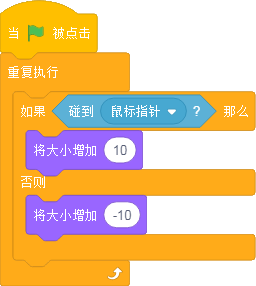
\includegraphics[width=\textwidth]{22.png}
                \caption*{第22题}
            \end{minipage}
        \end{figure}

        % 18
        \item 上面是展开的纸盒,合成一个纸盒后是什么样的?(\qquad)
        \begin{tasks}(4)
            \task 
\includegraphics[width=.05\textwidth]{18a.png}
            \task 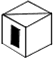
\includegraphics[width=.05\textwidth]{18b.png}
            \task 
\includegraphics[width=.05\textwidth]{18c.png}
            \task 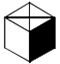
\includegraphics[width=.05\textwidth]{18d.png}
        \end{tasks}

        % 19
        \item 小猫坐标为$(0,0)$,点击绿旗执行上面程序,小猫有什么反应?(\qquad)
        \begin{tasks}(4)
            \task 移动
            \task 没有反应
            \task 说“走”
            \task 移动并说走
        \end{tasks}

        % 20
        \item 小芳、小明、小强三人去买铅笔,有红、绿两种颜色可以选择,小明说选红色的,小芳说不选绿色的,小强和小明选的不一样,下面说法不正确的是?(\qquad)
        \begin{tasks}(2)
            \task 小强选的是绿色
            \task 有两个人选了红色
            \task 有两个人选了绿色
            \task 小芳和小明选的颜色一样
        \end{tasks}

        % 21
        \item 如上图所示,根据小猫在舞台中的位置判断它$x,y$坐标的正负?(\qquad)
        \begin{tasks}(4)
            \task 正,负
            \task 正,正
            \task 负,负
            \task 负,正
        \end{tasks}

        % 22
        \item 执行如上图所示程序,什么时候角色会变小?(\qquad)
        \begin{tasks}(2)
            \task 鼠标指针移动到角色上时
            \task 鼠标指针从角色上移开时
            \task 点击鼠标时
            \task 松开鼠标时
        \end{tasks}

        \newpage
        % 23
        \item 角色位于$(-240,0)$,下面程序不能将角色移动到$(0,180)$的是?(\qquad)
        \begin{tasks}(4)
            \task 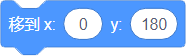
\includegraphics[width=.1\textwidth]{23a.png}
            \task 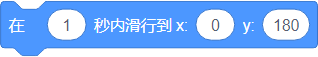
\includegraphics[width=.18\textwidth]{23b.png}
            \task 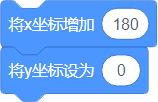
\includegraphics[width=.1\textwidth]{23c.png}
            \task 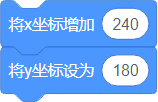
\includegraphics[width=.1\textwidth]{23d.png}
        \end{tasks}

        % 24
        \item 下列关于声音的说法不正确的是?(\qquad)
        \begin{tasks}(2)
            \task 一个角色只能有一个声音
            \task 背景和角色都可以添加声音
            \task 可以将声音进行反转操作
            \task 可以将声音进行机械化操作
        \end{tasks}

        % 25
        \item 点击绿旗,如下图所示程序可以画出什么图形?(\qquad)
        \begin{tasks}(4)
            \task 直线
            \task 虚线
            \task 破折线
            \task 波浪线
        \end{tasks}
    \end{enumerate}

    % 判断题
    {\noindent\textbf{第二部分、判断题(共 10 题,每题 2 分,共20分.)}}
    \begin{enumerate}
        \setcounter{enumi}{25}
        % 26
        \item 下面两个程序的运行结果是一样的.(\qquad)

        %27
        \item 新建作品,运行下面程序,角色会在舞台上画出一个组细为“5”的正六边形.(\qquad)
        
        \begin{figure}[htbp]
            \centering
            \begin{minipage}[t]{.11\textwidth}
                \centering
                \includegraphics[width=\textwidth]{25.png}
                \caption*{第25题}
            \end{minipage}
            \begin{minipage}[t]{.36\textwidth}
                \centering
                \begin{minipage}[t]{.45\textwidth}
                    \centering
                    \includegraphics[width=\textwidth]{26-1.png}
                \end{minipage}
                \begin{minipage}[t]{.5\textwidth}
                    \centering
                    \includegraphics[width=1\textwidth]{26-2.png}
                \end{minipage}
                \caption*{第26题}
            \end{minipage}
            \begin{minipage}[t]{.12\textwidth}
                \centering
                \includegraphics[width=\textwidth]{27.png}
                \caption*{第27题}
            \end{minipage}
            \begin{minipage}[t]{.2\textwidth}
                \centering
                \includegraphics[width=\textwidth]{28.png}
                \caption*{第28题}
            \end{minipage}
            \begin{minipage}[t]{.18\textwidth}
                \centering
                \includegraphics[width=\textwidth]{29.png}
                \caption*{第29题}
            \end{minipage}
        \end{figure}
        
        %28
        \item 上面两个程序的运行结果是一样的.(\qquad)

        %29
        \item 执行上面程序,当鼠标碰到角色时,角色停止移动.(\qquad)
        
        %30
        \item “苹果落地消失”游戏中,积木只能使用调整颜色值、饱和度值和亮度值的方法设置颜色.(\qquad)
        
        %31
        \item 程序前三次运行结果如A,B,C所示,根据图形推理第四次运行结果是E.(\qquad)
        
        \begin{figure}[htbp]
            \centering
            \begin{minipage}[t]{.24\textwidth}
                \centering
                \includegraphics[width=\textwidth]{30-3.png}
                \caption*{第30题}
            \end{minipage}
            \begin{minipage}[t]{.4\textwidth}
                \centering
                \begin{minipage}[t]{.55\textwidth}
                    \centering
                    \includegraphics[width=\textwidth]{31-1.jpg}
                \end{minipage}
                \begin{minipage}[t]{.4\textwidth}
                    \centering
                    \includegraphics[width=1\textwidth]{31-2.jpg}
                \end{minipage}
                \caption*{第31题}
            \end{minipage}
            \begin{minipage}[t]{.15\textwidth}
                \centering
                \includegraphics[width=\textwidth]{32.png}
                \caption*{第32题}
            \end{minipage}
            \begin{minipage}[t]{.15\textwidth}
                \centering
                \includegraphics[width=\textwidth]{33.png}
                \caption*{第33题}
            \end{minipage}
        \end{figure}

        %32
        \item 运行下面程序,播放“喵”10次.(\qquad)
        
        %33
        \item 执行下面程序,一直按空格键,角色顺时针旋转.(\qquad)
        
        %34
        \item 积木\includegraphics[width=.25\textwidth]{34.png}的结果为“true”.(\qquad)
        
        \newpage
        %35
        \item 下面三段程序分别是背景、鸭子、小猫的程序,点击绿旗,当按下空格键小猫叫两声之后,所有角色和背景声音都会停止.(\qquad)
        \begin{figure}[htbp]
            \centering
            \begin{minipage}[t]{.2\textwidth}
                \centering
                \includegraphics[width=\textwidth]{35-1.png}
            \end{minipage}
            \begin{minipage}[t]{.25\textwidth}
                \centering
                \includegraphics[width=1\textwidth]{35-2.png}
            \end{minipage}
            \begin{minipage}[t]{.19\textwidth}
                \centering
                \includegraphics[width=\textwidth]{35-3.png}
            \end{minipage}
            \begin{minipage}[t]{.15\textwidth}
                \centering
                \includegraphics[width=1\textwidth]{35-4.png}
            \end{minipage}
            \caption*{第35题}
        \end{figure}
    \end{enumerate}

    {\noindent \textbf{第三部分、编程题(共 2 题,共30分.)}}
    \begin{enumerate}
        \setcounter{enumi}{35}
        
        % 36
        \item 绘制图形:
        \begin{figure}[htbp]
            \begin{minipage}{.6\textwidth}
                1. 准备工作
                \begin{tasks}[label = (\arabic*)]
                    \task 隐藏小猫角色,默认舞台。
                \end{tasks}
                2. 功能实现
                \begin{tasks}[label = (\arabic*)]
                    \task 初始设定小猫中心点的坐标为$(x=0,y=0)$;
                    \task 线条粗细2,线条颜色为红色,每个正方形的边长为50;
                    \task 画出所示图形。
                \end{tasks}
            \end{minipage}
            \begin{minipage}{.37\textwidth}
                \centering
                \includegraphics[width=\textwidth]{36.png}
            \end{minipage}
        \end{figure}

    %     \newpage
        %37
        \item 货运飞船:
        \begin{figure}[htbp]
            \begin{minipage}{.6\textwidth}
                1. 准备工作
                \begin{tasks}[label = (\arabic*)]
                    \task 导入背景Galaxy;
                    \task 导入角色Rocketship、Block-A、Block-B、Block-C;
                    \task 绘制角色1、2、3为黑色小圆,代表太空垃圾。
                \end{tasks}
                2. 功能实现
                \begin{tasks}[label = (\arabic*)]
                    \task 点击绿旗,角色的初始位置如图所示,太空垃圾在宇宙中游荡;
                    \task 用上、下、左、右键,调整坐标控制货运飞船水平垂直飞行,不需要调整面向方向;
                    \task 飞船碰到太空垃圾将会消失,任务失败,停止全部脚本;
                    \task 飞船抵达角色Block-A、Block-B、Block-C位置,三个角色分别消失,表示货物已送达。
                \end{tasks}
            \end{minipage}
            \begin{minipage}{.37\textwidth}
                \centering
                \includegraphics[width=\textwidth]{37.jpg}
            \end{minipage}
        \end{figure}
    \end{enumerate}
\end{document}